\section{Формулы Френеля и угол Брюстера}

Из 1 эескремента у меня остались значения углов для 
поляризатор оностительно стекла, поэтому ставим в положение когда достигется 
минимум, а это значит, что нправление поляризатора перпендикулярно плоскости поляризатора,
и теперь начинаем вращать зеркало. 
\subsection{p}
\begin{figure}[h]
    \centering
    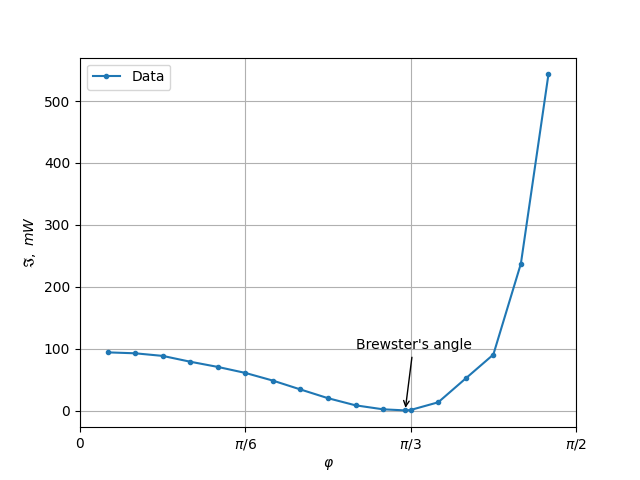
\includegraphics[trim={0 0 0 0},clip,width=\textwidth]{Ex_2/Task_2_1_1.png}
     \caption{Результаты измерений}
    \label{Task_2_1_1}
\end{figure}

Аппроксмирум данные формулой Френеля для положения p.
\begin{figure}[h]
    \centering
    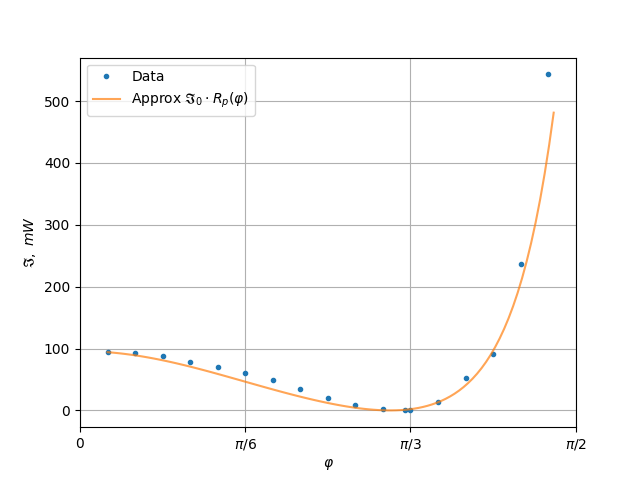
\includegraphics[trim={0 0 0 0},clip,width=\textwidth]{Ex_2/Task_2_1_2.png}
     \caption{}
    \label{Task_2_1_2}
\end{figure}
Я получил $$ n_1 = 1, n_2 = 1.5 $$

\subsection{s}
\begin{figure}[h]
    \centering
    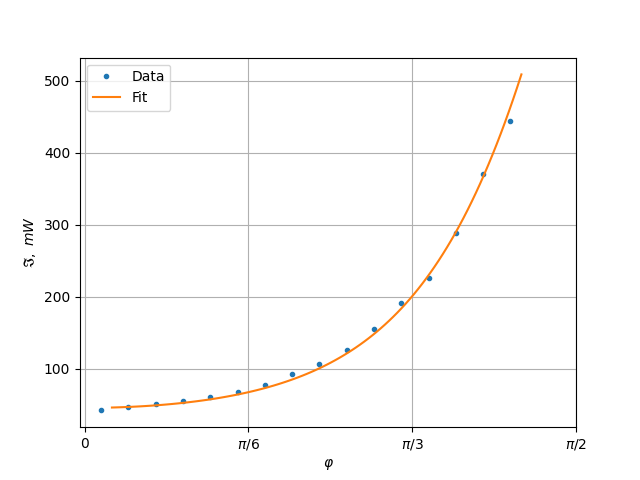
\includegraphics[trim={0 0 0 0},clip,width=\textwidth]{Ex_2/Task_2_2_1.png}
     \caption{Результаты измерений, c приближением}
    \label{Task_2_2_1}
\end{figure}

Я получил $$ n_1 = 1.01, n_2 = 1.93 $$





